\subsection{Descripción del Sistema}

Para el desarrollo de un sistema de visión artificial para vehículos autónomos no tripulados, se está diseñando un sistema capaz de recibir estímulos externos, interpretarlos y realizar acciones precisas y controladas en todos los actuadores, dando prioridad a la seguridad y la eficiencia. Por este motivo se hace imposible diseñar un autómata que contemple todos los posibles escenarios a los que podría estar sometido,por consiguiente se ha optado por desarrollar cada uno de los siguientes componentes.\\

\paragraph{Segmentación, localización y reconocimiento de imágenes}
El procesamiento de imágenes representa un componente fundamental, es el sistema encargado de dotar con percepción al agente simulado. Para llevar a cabo esta tarea se ha optado por desarrollar un algoritmo de segmentación de imágenes por regiones, esto debido a su bajo costo computacional, respecto a técnicas basadas en bordes o puntos de interés. En concreto se está implementando una hibrido de los algoritmos K-nearest neighbors y DBSCAN (Density-Based Spatial Clustering of Applications with Noise). En la figura \ref{ejemclust} puede verse ejemplos de estos algoritmos.\\

\begin{itemize}
	\item \textbf{K-nearest neighbors:} En este algoritmo se decide la membresia de un objeto teniendo en cuenta sus vecinos. Se decide a que cluster pertenece mirando a que cluster pertenece la mayoría de sus vecinos K más cercanos a el \cite{cluster}.\\
	
	\item \textbf{DBSCAN:} Es un algoritmo de clustering creado en 1996, no paramétrico, basado en densidades, y que marca como outliers aquellos puntos que no superan un umbral de densidad establecido \cite{cluster2}.\\
\end{itemize}

\begin{figure}
	\begin{center}
		\begin{subfigure}{0.49\textwidth}
			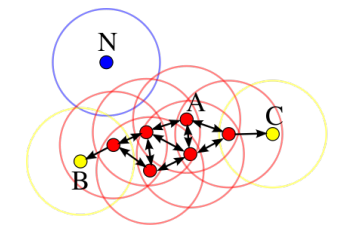
\includegraphics[width=\textwidth]{images/DBSCAN.png}
			\caption{DBSCAN: En este caso el mínimo numero de puntos es P = 3. Los puntos de A todos contienen al menos 3 puntos en un radio E y por ello forman un cluster. Tanto B como C son alcanzables desde A por lo que formaran parte del cluster, son el limite de este. N es un nodo ruidoso, no es alcanzable por ningún punto \cite{cluster}.\\}
		\end{subfigure}
		\begin{subfigure}{0.49\textwidth}
			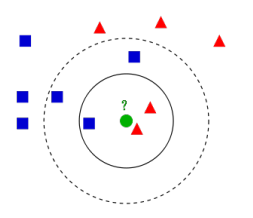
\includegraphics[width=\textwidth]{images/nearest.png}
			\caption{K-nearest: El circulo verde debería ser clasificado con los azules o rojos según el numero K de vecinos que escojamos. Si k=3 sera asignado al rojo ya que	de sus 3 vecinos mas cercanos dos son rojos. Si k=5 ira al azul al tener tres vecinos azules y dos rojos \cite{cluster}.}
		\end{subfigure}
	\end{center}
	\caption{Ejemplo de algoritmos de clustering }\label{ejemclust}
\end{figure}

El algoritmo propuesto consiste en los siguientes pasos:\\

\begin{enumerate}
	\item Partimos de un pixel y miramos si desde ese punto hay un mínimo de puntos P en un radio de distancia E, se considera que hay un punto P cuando el pixel cumple con una regla difusa para determinar su parecido en el espacio de color HSL.
	\item Si es así, esto forma un cluster y volvemos a la etapa 1 con un punto no explorado.
	\item Si no encontramos el mínimo de puntos pero hemos llegado a ese punto a través de un punto que si lo cumplía, éste formará parte del cluster. En caso de no poder llegar a un punto a través de otros no formará	parte del cluster y será un nodo ruidoso.\\
\end{enumerate}

		\paragraph{Estimación de la distancia.}
		Luego de tener la imagen segmentada correctamente se debe establecer un mapa de disparidad, utilizando visión binocular para calcular la disparidad horizontal, como indicativo de la distancia aproximada de los objetos en la escena. El proceso de clustering realizado anteriormente servirá como correspondencia, para identificar las zonas del mismo objeto a calcular su disparidad. Conociendo la disposición geométrica de las cámaras, se puede conocer la distancia a la que se encuentran los puntos de interés utilizando triangulación. Las imágenes deben estar rectificadas, consiste en que las filas de las imágenes izquierda y derecha estén alineadas, de esta manera dado un punto de interés en la imagen izquierda, su punto correspondiente en la imagen derecha se encontrara en la misma fila en ambas imágenes. Utilizando la ecuación \ref{eq:disparidad_calculo} puede encontrarse la distancia $Z$ donde $f$ corresponde a la longitud focal, $T$ a la distancia entre las cámaras, donde  coordenadas en el eje horizontal son respectivamente $x^l$ y $x^r$. Ver figura \ref{fig:stereo_pair}.

		\begin{figure}
			\begin{center}
				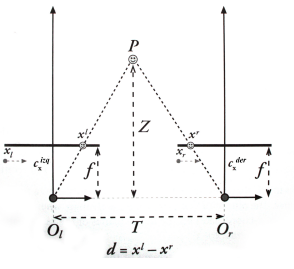
\includegraphics[width=0.45\textwidth]{images/disparidad.png}\\
				\caption{Par estéreo perfectamente reajustado, rectificado y con una correspondencia conocida, la distancia Z se puede encontrar mediante triángulos semejantes.}\label{fig:stereo_pair}
			\end{center}
		\end{figure}

		\begin{figure}
			\begin{center}
				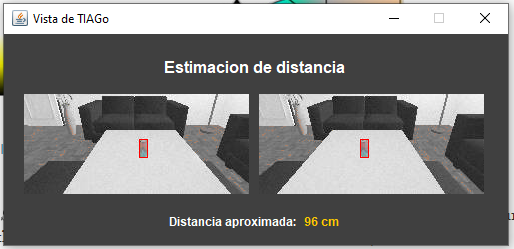
\includegraphics[width=0.45\textwidth]{images/estimacion.png}\\
				\caption{Estimación de distancia realizada con la ecuación \ref{eq:disparidad_calculo} con un par binocular. En el entorno de simulación Webots}\label{fig:distance_estimation}
			\end{center}
		\end{figure}

		\begin{equation} \label{eq:disparidad_calculo}
			Z=\frac{fT}{x^l - x^r}
		\end{equation}

		El algoritmo propuesto para determinar la distancia consiste en los siguientes pasos:\\

		\begin{enumerate}
			\item Recorrer la imagen izquierda, distinguiendo los clusters presentes en cada fila.
			\item Para cada fila verificar los clusters e identificar el cluster correspondiente en la misma fila en la imagen derecha.
			\item Calcular la disparidad con la ecuación \ref{eq:disparidad_calculo} cuando se encuentre la correspondencia.
			\item Modificar la imagen a un gris equivalente a su profundidad, siendo desde blanco puro a objetos muy cercanos, y negro puro para objetos sin disparidad horizontal.\\
		\end{enumerate}

		\paragraph{Digitalización del entorno.}
		La digitalización del entorno consiste el identificar los objetos con una disparidad todavía por determinar, que se encuentren en el rango medio de profundidad, e inferir su tamaño real de acuerdo al tamaño relativo en la imagen, estos objetos serán representados en un mapa bidimensional visto desde arriba, como nodos negros identificando un obstáculo y nodos claros identificando espacio libre. Ver figura \ref{fig:environment_map}.

		\begin{figure}
			\begin{center}
				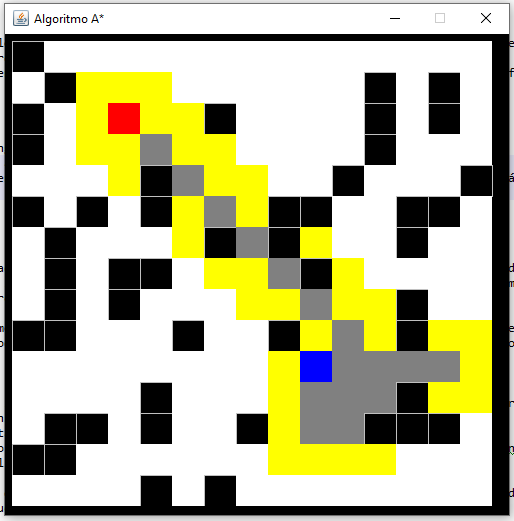
\includegraphics[width=0.45\textwidth]{images/astar.png}\\
				\caption{Mapa discretizado del mundo, generado aleatoriamente. Donde los nodos negros representan obstáculos, los nodos blancos representan espacio libre. El nodo rojo representa el punto de inicio del agente y el azul el punto de llegada, los demás colores son estados del algoritmo A-star}\label{fig:environment_map}
			\end{center}
		\end{figure}

		\paragraph{Algoritmo A* (A-star)}
		Este algoritmo es una mejora desarrollada a los postulados del algoritmo Dijsktra que se encarga de encontrar rutas más cortas dentro de un grafo. En esta modificación se toma como punto central la observación búsquedas informadas dentro del grafo que nos permitan tomar decisiones óptimas sobre los caminos que deben tomarse para recorrer de forma eficiente el grafo.

		En la figura \ref{fig:environment_map} puede verse el uso del algoritmo A*, implementado en java haciendo uso de listas para el manejo de los estados de cada nodo. Donde los nodos amarillos y grises representan todos los nodos explorados para encontrar la mejor ruta desde el punto A(rojo), al punto B(azul).

		\paragraph{Aplicativo de Inferencia Difusa.}
		Los aplicativo para inferencia difusa que se encuentra implementado actualmente se encarga de identificar los colores para el proceso de clustering, lo que hace es comparar dos colores y definir si son o no parecidos, para esta tarea se trabaja sobre el espacio de color HSL, debido a la gran semejanza que tiene respecto a la vista humana, donde dos colores del mismo tono pero con diferente saturación o luz se catalogarían parecidos para el pensamiento humano, pero el espacio de color RGB se encuentran mucho más alejas que en el HSL. En la figura \ref{fig:hsl} puede verse un esquema del mapa de color utilizado.

		Adicionalmente el controlador difuso será el encargado de accionar los actuadores del robot para$\$ desplazarse por la ruta obtenida con el algoritmo A*, siguiendo un esquema de diseño como el que puede verse en la figura.

		\begin{figure}
			\begin{center}
				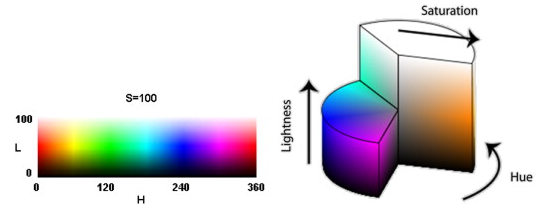
\includegraphics[width=0.49\textwidth]{images/hsl.png}\\
				\caption{Modelo de color HSL.}\label{fig:hsl}
			\end{center}
		\end{figure}

\begin{figure}
	\begin{center}
		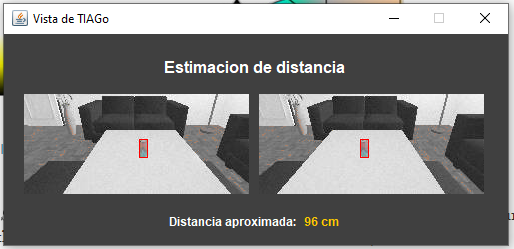
\includegraphics[width=0.45\textwidth]{images/estimacion.png}\\
		\caption{Estimación de distancia realizada con la ecuación \ref{eq:dispa} con un par binocular. En el entorno de simulación Webots}\label{disp2}
	\end{center}
\end{figure}

\begin{equation} \label{eq:dispa}
	Z=\frac{fT}{x^l - x^r}
\end{equation}

El algoritmo propuesto para determinar la distancia consiste en los siguientes pasos:\\

\begin{enumerate}
	\item Recorrer la imagen izquierda, distinguiendo los clusters presentes en cada fila.
	\item Para cada fila verificar los clusters e identificar el cluster correspondiente en la misma fila en la imagen derecha.
	\item Calcular la disparidad con la ecuación \ref{eq:dispa} cuando se encuentre la correspondencia.
	\item Modificar la imagen a un gris equivalente a su profundidad, siendo desde blanco puro a objetos muy cercanos, y negro puro para objetos sin disparidad horizontal.\\
\end{enumerate}

\paragraph{Digitalización del entorno.}
La digitalización del entorno consiste el identificar los objetos con una disparidad todavía por determinar, que se encuentren en el rango medio de profundidad, e inferir su tamaño real de acuerdo al tamaño relativo en la imagen, estos objetos serán representados en un mapa bidimensional visto desde arriba, como nodos negros identificando un obstáculo y nodos claros identificando espacio libre. Ver figura \ref{digi}.

\begin{figure}
	\begin{center}
		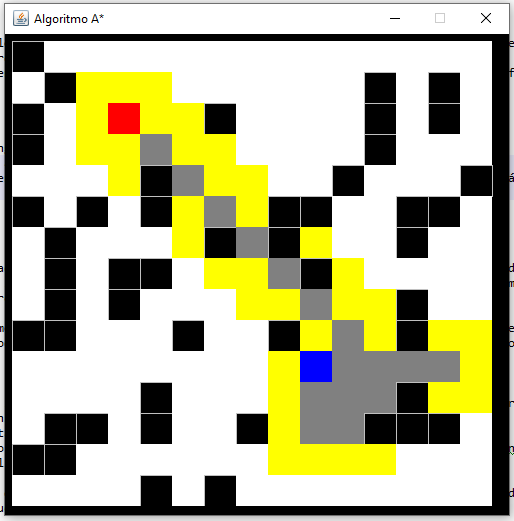
\includegraphics[width=0.45\textwidth]{images/astar.png}\\
		\caption{Mapa discretizado del mundo, generado aleatoriamente. Donde los nodos negros representan obstáculos, los nodos blancos representan espacio libre. El nodo rojo representa el punto de inicio del agente y el azul el punto de llegada, los demás colores son estados del algoritmo A-star}\label{digi}
	\end{center}
\end{figure}

\paragraph{Algoritmo A* (A-star)}
Este algoritmo es una mejora desarrollada a los postulados del algoritmo Dijsktra que se encarga de encontrar rutas más cortas dentro de un grafo. En esta modificación se toma como punto central la observación búsquedas informadas dentro del grafo que nos permitan tomar decisiones óptimas sobre los caminos que deben tomarse para recorrer de forma eficiente el grafo \cite{astar}.\\

En la figura \ref{digi} puede verse el uso del algoritmo A*, implementado en java haciendo uso de listas para el manejo de los estados de cada nodo. Donde los nodos amarillos y grises representan todos los nodos explorados para encontrar la mejor ruta desde el punto A(rojo), al punto B(azul).\\

\paragraph{Aplicativo de Inferencia Difusa.}
Los aplicativo para inferencia difusa que se encuentra implementado actualmente se encarga de identificar los colores para el proceso de clustering, lo que hace es comparar dos colores y definir si son o no parecidos, para esta tarea se trabaja sobre el espacio de color HSL, debido a la gran semejanza que tiene respecto a la vista humana, donde dos colores del mismo tono pero con diferente saturación o luz se catalogarían parecidos para el pensamiento humano, pero el espacio de color RGB se encuentran mucho más alejas que en el HSL. En la figura \ref{hsl} puede verse un esquema del mapa de color utilizado.\\

Adicionalmente el controlador difuso será el encargado de accionar los actuadores del robot para$\\$ desplazarse por la ruta obtenida con el algoritmo A*, siguiendo un esquema de diseño como el que puede verse en la figura \cite{controlador}.

\begin{figure}
	\begin{center}
		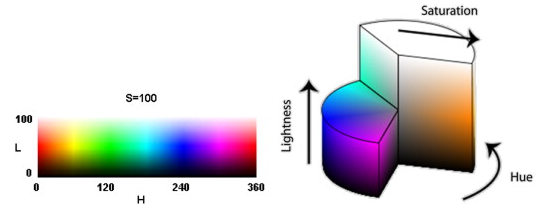
\includegraphics[width=0.49\textwidth]{images/hsl.png}\\
		\caption{Modelo de color HSL \cite{hsl}.}\label{hsl}
	\end{center}
\end{figure}